\chapter{Optimierung des DSP-Codes}
\label{ch:optdsp}
\rm

In diesem Kapitel soll die Planung und Optimierung des DSP-Codes beschreiben werden.\\
Wie bereits in \textbf{Kapitel \ref{sec:ansatz}} gezeigt wurde, nimmt die Extraktion der zu untersuchenden Features einen Gro�teil der Laufzeit des Programmes ein.
Unter diesem Gesichtspunkt und der in \textbf{Kapitel \ref{sec:davinci}} gezeigten zugrundeliegenden heterogenen Architektur des zu betrachtenden Systems, liegt es nahe, die Extraktion auf dem DSP auszuf�hren.\\
In den nun folgenden Abschnitten sollen daher, wie schon im vorhergehenden Kapitel erst die Bottlenecks identifiziert (\textbf{\ref{sec:ansatzdsp}}) und danach die durchgef�hrten Optimierungen beschrieben werden (\textbf{\ref{sec:mathlib}} - \textbf{\ref{sec:compiler}}).

\section{Bottlenecks des DSP-Codes}\label{sec:ansatzdsp}

F�r die Laufzeitmessungen des DSP-Codes wurden wie schon im vorherigen Kapitel die FeaturesSets 1-4 (\textbf{\ref{subsec:fset1}} - \textbf{\ref{subsec:fset4}}) verwendet.
Die ben�tigen Zeiten wurden auch hier wieder mit der Gesamtzeit in Verh�ltnis gesetzt, wodurch die aus \textbf{Abbildung \ref{fig:dsp}} zu entnehmenden Anteile der einzelnen Features an der Gesamtlaufzeit errechnet wurden.

\begin{figure}
	\centering
		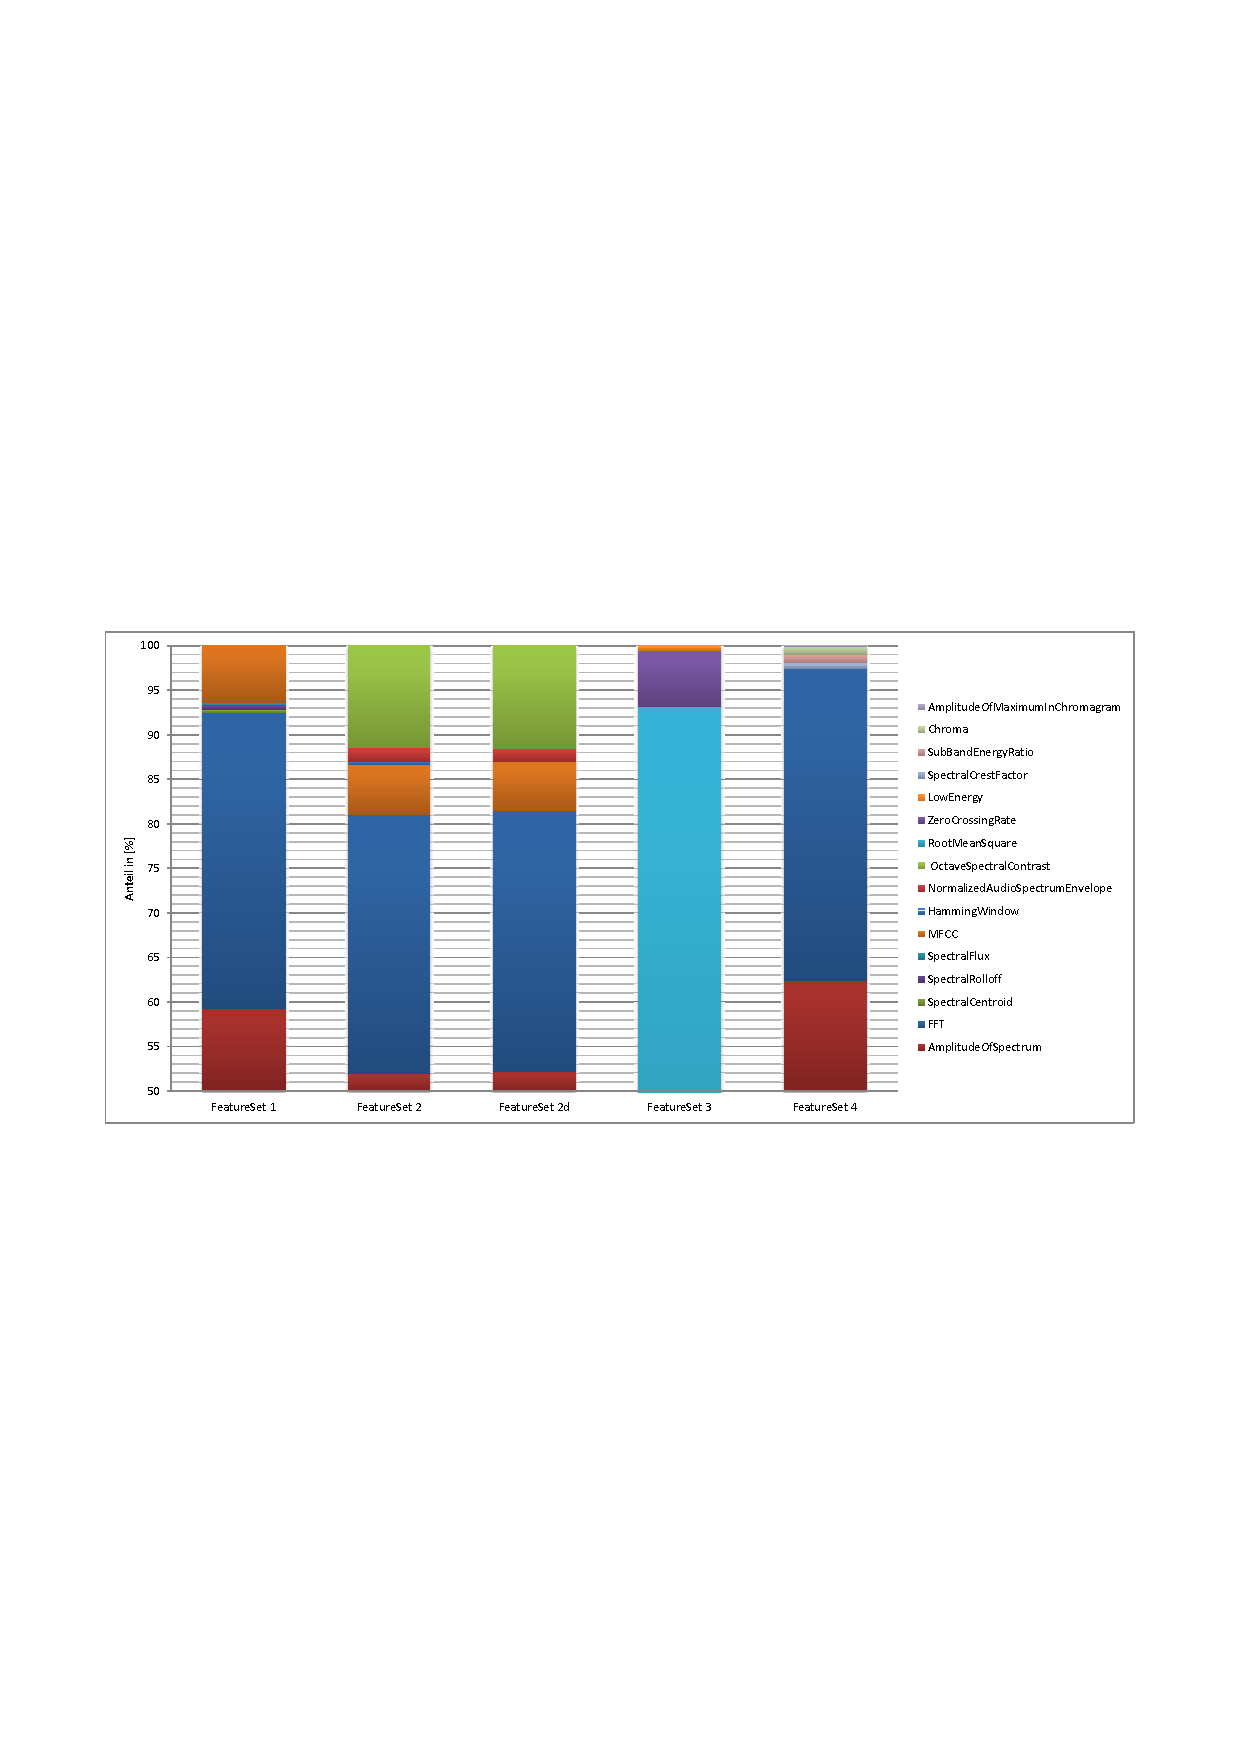
\includegraphics[width=1.00\textwidth]{../Pictures/ResultsExtraktionDSP.pdf}
	\caption{Laufzeitanteile der Features auf dem DSP}
	\label{fig:dsp}
\end{figure}

Es ist deutlich zu erkennen, dass in den FeatureSets 1 - 2d und 4 \textit{Amplitude of Spectrum} (\textbf{\ref{subsubsec:aos}}) und im FeatureSet 3 \textit{Root Mean Square} (\textbf{\ref{subsubsec:rms}}) die meiste Laufzeit in Anspruch nehmen, teilweise mit Anteilen weit �ber 50\%. Da beide Features eigentlich nur aus Summationen, Divisionen und der Bildung von Quadratwurzeln bestehen, die Bestandteil der Standartbibliotheken sind, scheint bei der Ausf�hrung von mathematischen Funktionen ein Bottleneck zu entstehen. Des weiteren ist zu sehen, dass auch bei der Umsetzung des Codes auf dem DSP ein weiterer Bottleneck bei der Ausf�hrung der FFT zu bestehen scheint, da auch diese mit ca. 30\% der Ausf�hrungszeit zu Buche schl�gt.

\section{Optimierung der Rechenfunktionen mit MATHLIB}\label{sec:mathlib}

\section{Optimierung der FFT mit DSPLIB}\label{sec:dsplib}

\section{Optimierung f�r den Compiler}\label{sec:compiler} 